

\chapter{Deep learning in archaeology}

\begin{introduction}
In this chapter, it will be discussed various ways of applying artificial intelligence models to archaeology.
\end{introduction}
Remote sensing is the technique of obtaining information about an object, an area, or a phenomenon without direct contact between the sensor and the object or area being observed.

Its use dates back to the early 20th century\cite{asmr}, and it was then used heavily for military purposes during World War I (1914-1918)\cite{war1}, when airplanes were equipped with cameras. The information recorded in the photographs was used for target recognition and military planning.
Later, this type of technique was widely spread in civil society, where it was used for various purposes. 

In the field of this dissertation, its use is for the purpose of indicating geographical regions likely to contain archaeological objects.

%As mentioned before, we do not use cameras, but LIDAR (laser imaging, detection, and ranging) technique. LIDAR is a sensor that emits laser beams in the infrared band and is able to model the ground surface three-dimensionally, making it a powerful tool for archaeology. This technique will be discussed in more detail further below.


\section{Airborne and Spaceborne Remote sensing}

Preservation of \ac{ach} is a critical strategic priority aiming to protect and transmit cultural artifacts and historical evidence to future generations.

Remote sensing from elevated points was initially used in the field of ACH\cite{asmr}, marking one of its pioneering applications.

In the field of ACH, remote sensing usually refers to all techniques that use non-direct contact to observe areas of interest on Earth.

More than a century has passed since the inception of airborne remote sensing in the field of ACH around 1900. Dating back to 1839, with the birth of photography, photographers had attempted to lift cameras to capture aerial perspectives of the Earth's surface.

In 1906, a British general used a military hot air balloon to take vertical and oblique photographs of the Stonehenge site. After the 1900s, the majority of aerial photographs were taken from airplanes, revolutionizing the perspective from which images were captured above the Earth's surface.


\subsection{Photography}
The use of photography in archaeology has become more common in the last 110 years\cite{asmr}, as one of the methods that allows the discovery of archaeological sites after they have been destroyed, either by man or by natural phenomena. 

There are traces of ancient, man-made transformations of the landscape that can only be seen from above, and this is where photograrchaeology comes in.

\begin{figure}[h]
\centering
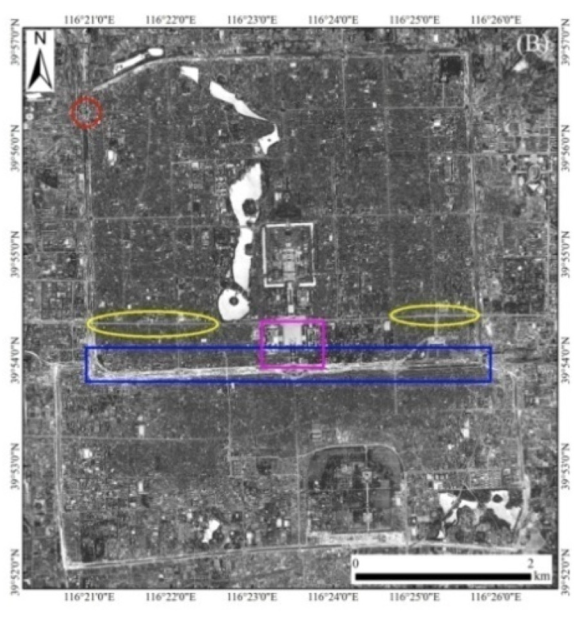
\includegraphics[height=7cm]{images/foto.png}
\caption[Aerial photograph in 1945 of Beijing]{Aerial photograph in 1945 of Beijing \cite{asmr}}
\end{figure}

\subsection{Hyperspectral and multispectral image}
Unlike photography, which uses only frequencies within the visible range, hyperspectral and multispectral imaging uses a wider range of frequencies that are not visible to the naked eye.


Multispectral has wavelengths usually between the visible and infrared and typically uses 3 to 15 bands with a length greater than 20 nm. An example of the use of multispectral imagery is the Landsat-8 satellite, which produces 11 images from different bands, all but 3 of which have a resolution of 30 meters.

The images  \ref{olisensors} and \ref{tirssensors} show the different bands used in Landsat-8 imagery.

\begin{figure}[H]
\centering
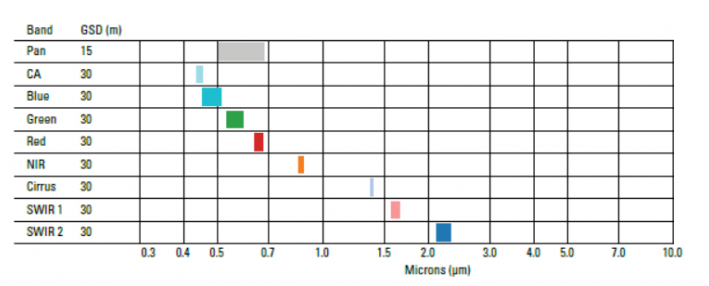
\includegraphics[width=14cm]{images/landsat1.png}
\caption[Landsat-8 bands from the OLI sensor]{Landsat-8 bands from the OLI sensor\cite{landsat}}
\label{olisensors}
\end{figure}

\begin{figure}[H]
\centering
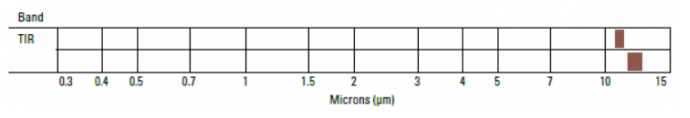
\includegraphics[width=14cm]{images/landsat2.png}
\caption[Landsat-8 bands from the TIRS sensor]{Landsat-8 bands from the TIRS sensor\cite{landsat}}
\label{tirssensors}
\end{figure}

Hyperspectral imaging, on the other hand, typically uses hundreds or thousands of narrower bands (typically smaller than 20nm).

These fundamental differences between multispectral and hyperspectral imaging have a major impact on archaeological prospecting, since the more and narrower the bands, the greater the ability to detect subtly different spectral reflections in the ground.

It is also worth mentioning that buried archaeological objects can have their chemical, physical and biological properties altered, causing differences in spectral reflectance.


\subsection{LiDAR}
LiDAR has become an essential part of archaeological prospecting. By attaching it to a drone, for example, it is possible to cover large areas in order to discover new sites with archaeological potential.  Its operation is based on emitting high-frequency light beams and then measuring the time it takes for the light beam to reach the object and return.
By analyzing the characteristics of the returned signal, it is possible to create a 3D map of the area in question.

The image \ref{Point cloud from Viana do Castelo} shows an example of a point cloud from an area in Viana do Castelo.

\begin{figure}[H]
\centering
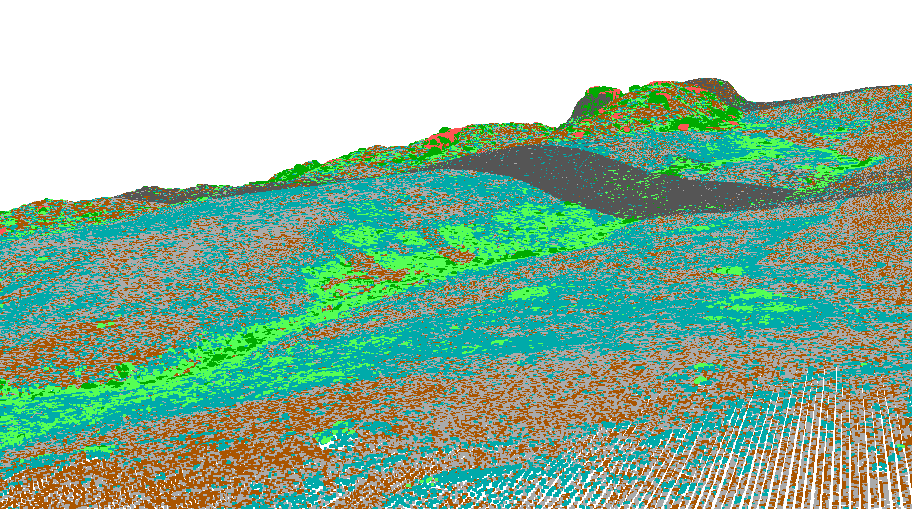
\includegraphics[width=10cm]{images/pointcloudViana.png}
\caption{Point cloud from Viana do Castelo}
\label{Point cloud from Viana do Castelo}
\end{figure}

In the image each color of the point represents the category the point belongs to - for example green represents vegetation and brown represents soil.

As a result of the work of archaeologists and specialists, airborne lidar has been successfully used to detect archaeological features around the world. However, in order to be useful, it is first necessary to classify and fit the points in the point cloud, which is a crucial process to identify and remove points that do not belong to the ground in order to be able to detect archaeological features. The result of this filtering is called a \ac{dtm}. However, it should be noted that this method is not perfect and it is possible to filter too much, in this case filtering points that belong to archaeological objects.

The image \ref{Point cloud from Viana do Castelo filtered} shows the same zone but filtered showing only the points classified as soil.
\begin{figure}[H]
\centering
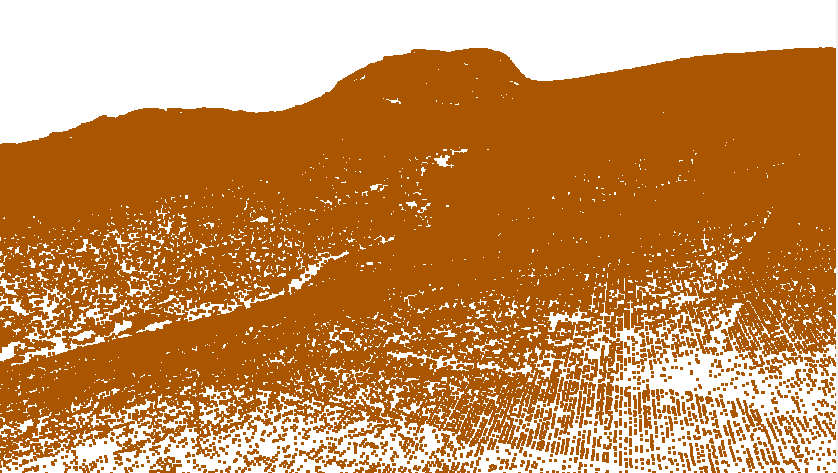
\includegraphics[width=10cm]{images/pointcloudVianafiltrado.png}
\caption{Point cloud from Viana do Castelo filtered}
\label{Point cloud from Viana do Castelo filtered}
\end{figure}

\section{Relief Visualization Techniques}

For the implementation of deep learning algorithms, one of the possibilities is to use directly the filtered Lidar radar data, i.e. to use the \ac{dtm}, as it is shown in the article \cite{deeplearningRawLidarData}. However, deep learning methods may have certain limitations, as many human resources are needed to make the annotations. In the case of archaeological annotations, if done by non-professionals, they may contain errors due to lack of knowledge of the scene and structure of the object in question. 

Another option is to pre-process the point cloud to create an image with the relief information. There are several techniques to create such images. In the article\cite{reliefModel} 13 methods are listed. However, we will only discuss the two most effective according to the article, e2MSTP and MSTP, and the LRM used in the thesis.

\subsection{MSTP and Enhanced MSTP}
One of the most efficient techniques used is \ac{mstp}. As explained in \cite{mstp}, it works well for visual interpretation and semi-automatic feature detection. By focusing on the topographical context of the structures rather than the structures themselves, it is particularly good for heterogeneous objects. Enhanced MSTP adds a morphological visualization technique to MSTP, creating a more detailed image.

The image \ref{MSTP and Enhanced MSTP} shows an MSTP image, a morphological visualization, and the result of combining the two, the enhanced MSTP image.

\begin{figure}[H]
\centering
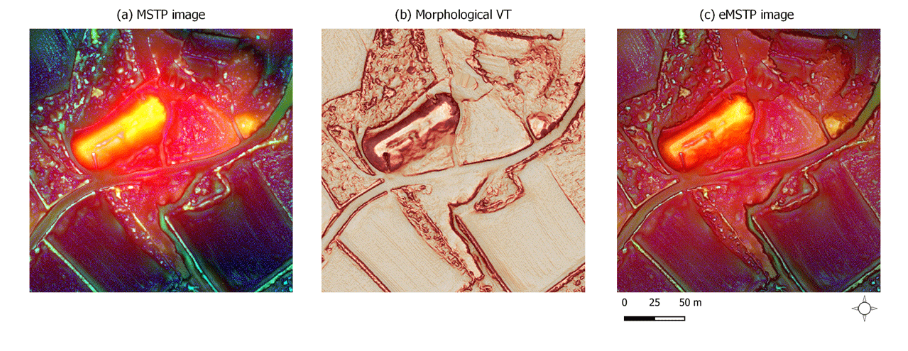
\includegraphics[width=\textwidth]{figs/mstp.png}
\caption[MSTP and Enhanced MSTP]{MSTP and Enhanced MSTP \cite{emstp}}
\label{MSTP and Enhanced MSTP}
\end{figure}

It is important to note that this technique does not provide topographical measurements since the RGB values do not represent elevations or slopes.

According to \cite{emstp}, enhanced MSTP allowed researchers to obtain a detection accuracy of 77\%, proving thia to be a good technique especially if combined with the right deep learning model.

\subsection{Local relief model (LRM)}

Local Relief Model (LRM) is one of the most widely used techniques for archaeological purposes. In \ac{lrm} small-scale elevation differences are represented after the landscape is removed from the data, as in \ac{dtm}. 

The LRM significantly improves the detectability of shallow, small-scale topographic features, regardless of the lighting conditions. It enables direct measurement of both their relative heights and volumes\cite{lrm}.

When a low-pass filter is applied to the \ac{dtm}, it results in a smoothed elevation model, which serves as an initial representation of the large-scale landscape forms. The size of the kernel used in the low-pass filter determines the spatial scale of features captured in \ac{lrm}.

\section{Deep learning VS Machine Learning}

This section explains how it is possible to apply both deep learning and machine learning methods to archaeology.

Since LRM imaging is one of the most widely used techniques in archaeology, a logical next step is to apply deep learning methods to the detection of new archaeological sites. These methods can be objection detection or semantic segmentation. Both methods are based on CNN (Convolutional Neural Network).

\subsection{Convolution Neural Network }
\ac{cnn} is one of the most recurrent forms of deep learning because it is based on the human brain. Unlike classical machine learning, where it is necessary to first collect features from the dataset and then feed them into the machine learning algorithm, CNNs are also able to train filters that can extract these features.

The operation is based on an input layer, where the image passes through several convolution layers.
The convolution layer applies a set of filters or kernels to the input image, each of which extracts a specific feature from the image. For example, one filter might detect horizontal edges, another filter might detect vertical edges, and so on. The filter is moved over the input image, performing a point-to-point multiplication at each position, and the average of the sums of these multiplications is calculated to produce an output value at a given position. At the end, a feature map is created.

Between each convolution layer, it is normal to have a polling layer, which is used to reduce the size of the feature map to reduce the number of features. This layer divides the image into rectangular regions, and then for each region, simply takes the highest value or averages the values.
After the last max-poling layer come the dense layers, but for this you need to transform the image from matrix to vector, and for this a flatten layer is used.

The dense layers, also known as fully connected layers, are used to process the data from the previous layers.

Finally, we have the output layer, which can be a sigmoid if the result is binary, or a softmax if it is not.

\begin{figure}[H]
\centering
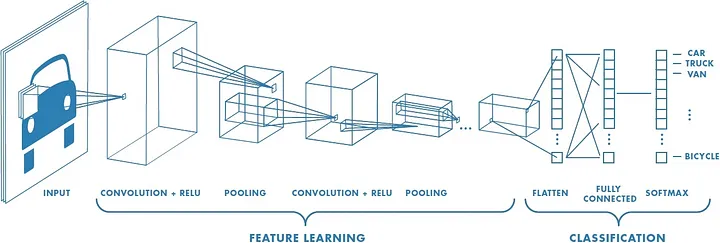
\includegraphics[width=15cm]{images/cnn.png}
\caption[Example of neural network]{Example of neural network \cite{mediumCNN}}
\end{figure}

\subsection{Machine Learning}
The main difference between deep learning and machine learning lies in the architecture and the level of complexity in the learned tasks. One notable distinction is the degree of human involvement. In deep learning, the model learns to extract features from the data on its own, while in traditional machine learning, humans need to manually extract features from the data and then provide them as input to the algorithm.

\begin{figure}[H]
\centering
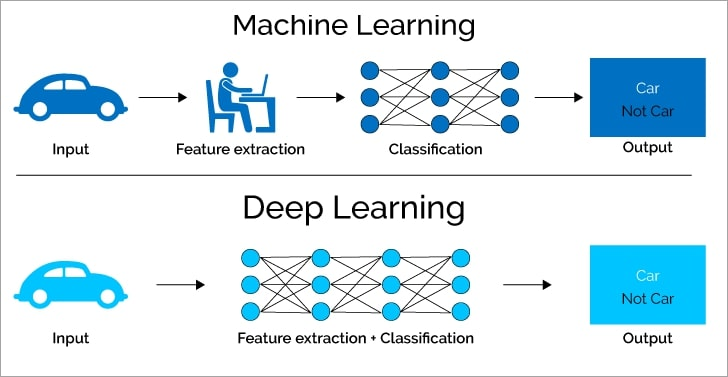
\includegraphics[width=15cm]{images/deepLearningVSmachineLearning.jpeg}
\caption[Machine Learning VS Deep learning]{Machine Learning VS Deep learning\cite{deepLearningVSmachineLearning}}
\end{figure}

The use of machine learning methods in archaeology using the \ac{lidar} data without preprocessing is a technique that has been used. The unsupervised clustering based machine learning methods are more suitable for irregular object\cite{deeplearningRawLidarData}.

When it comes to cultural heritage, surface or structural defects often appear in the form of irregular geometric features. These can include weathering, cracks, and partial defects. As a result, these algorithms are exceptionally well suited for identifying and extracting surface defects in such cases\cite{deeplearningRawLidarData}.